\chapter{Computational aspects of Fluid-Structure Interaction problems}
\label{cha:computation}

This section deals with the computational aspects of FSI problems. The first possible categorization of solution techniques distinguishes between monolithic and partitioned approach, as discussed in Section \ref{sec:monolithic}. This work is based on the latter approach, so the two different coupling strategies, namely strong and weak, are discussed in Section \ref{sec:coupling}. As strong coupling is generally needed for accurate solution, ad overview of strong coupling algorithms is given in Section \ref{sec:strong-coupling}. Section \ref{sec:interface-mesh} focuses on aspects concerning the interface mesh, and how the solid and the fluid exchange data between them. Finally \ref{sec:addedd-mass} briefly describes a common issue arising in strongly coupled problems: the ~\ac{AME}.


\section{Monolithic and Partitioned Approach}
\label{sec:monolithic}

Analytical solutions are impossible to obtain for the large majority of FSI problems; on the other hand, laboratory experiments may be costly, unfeasible or limited. For those reasons, numerical simulations may be employed to analyze the physics involved in the interaction between fluids and solids. With the current capabilities of computer technology, simulations of scientific and engineering models have become increasingly detailed and sophisticated.

The numerical methods used to solve FSI problems may be roughly classified into two classes: the \textit{monolithic approach} and the \textit{partitioned approach}. There is no exact distinction between the two approaches, as they might be seen differently among fields of applications. The idea here is to consider how many solvers are used to find a solution.

In the \textit{monolithic approach}, the whole problem is treated as a unique entity and solved simultaneously with a specialized ad hoc solver (see Figure \ref{fig:monolithic}). The fluid and structure dynamics form a single system of equations for the entire problem, which is solved simultaneously by a unified algorithm. The interface conditions are implicit in the solution procedure \cite{hubner2004monolithic}, \cite{ryzhakov2010monolithic}.

This approach can potentially achieve better accuracy, as they solve the system of equations exactly the interface conditions are implicit in the model \cite{richter2017fluid}, but it may require more resources and expertise to develop from scratch a specialized code (it solves a very specific model) that can be cumbersome to maintain.

\begin{figure}[htbp!]
	\centering
	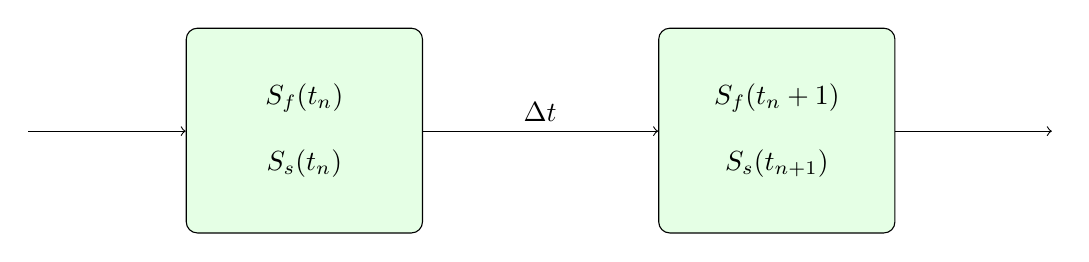
\begin{tikzpicture}[scale=1]


	\tikzstyle{status}=[draw,rectangle,rounded corners,fill=green!10,text centered,inner sep=10pt, anchor=south west, minimum width=3cm,minimum height=2.6cm]
	\draw[->] (0,1.3)-- (2,1.3) node[] {};
	
	\draw[->] (5,1.3)-- (8,1.3) node[midway,above] {$\Delta t$}; % node[midway,below] {step};

	\draw[->] (11,1.3)-- (13,1.3) node[] {};

	\node[status] (t1) at (2,0)  {
		\begin{tabular}{c}
			$S_f(t_n)$ \\
			\\
			$S_s(t_n)$
	\end{tabular}};

	\node[status] at (8,0) {
	\begin{tabular}{c}
		$S_f(t_{n}+1)$ \\
		\\
		$S_s(t_{n+1})$
\end{tabular}};
	
%		\draw (0,1.3) node[below] {$B$} --
%		(3,1.3) node[below] {$C$} --
%		(1.5,4.3) node[above] {$A$} -- cycle;
%		\draw (1.5,4.3) -- (1.5,1.3) node[below] {$D$};
%		\draw (1.5,1.5) -- (1.7,1.5) -- (1.7,1.3);
%		\node[draw,text width=3cm] at (4.5,4) {some text spanning three lines with automatic line breaks};
%		\draw[rounded corners=5pt] (4,0) rectangle ++(2,1);
	\end{tikzpicture}
	\caption{monolithic approach: $S_f$, $S_s$ denote the fluid and the structure solutions}
	\label{fig:monolithic}
\end{figure}


On the other hand, in the \textit{partitioned approach}, the fluid and the solid domains are treated as two distinct computational fields, with their respective meshes, that have to be solved separately (see Figure \ref{fig:partitioned}: how data are passed between solvers is detailed in Section \ref{sec:coupling}). The interface conditions are used explicitly to communicate information between the fluid and structure solutions. This implies that the flow does not change while the solution of the structural equations is calculated and vice versa \cite{degroote2009performance}. The partitioned approach thus requires a third software module (i.e. a coupling algorithm) to incorporate the interaction aspects. It communicates the boundary conditions described in Section \ref{sec:interface}: that is forces or stresses (dynamic data) calculated by the fluid solver at the wet surface are passed to the solid component and displacements or velocities (kinematic data) computed by the solid solver at the interface are sent to the fluid component in return. Finally, fluid and structural solutions together yield the FSI solution.

\begin{figure}[htbp!]
	\centering
	\begin{tikzpicture}[scale=1]

	\tikzstyle{solver}=[draw,rectangle,rounded corners,text centered,inner sep=10pt, anchor=south west, minimum width=3cm,minimum height=1.2cm]
	\tikzstyle{coupling}=[draw, ellipse, fill=yellow!75, minimum width=3cm, minimum height=1.2cm, align=center]

	\node[solver,fill=blue!20] at (2,4.4) {$S_f(t_n)$};
	\node[solver,fill=blue!20] at (8,4.4) {$S_f(t_{n+1})$};
	
	\node[solver,fill=orange!50] at (2,0) {$S_s(t_n)$};
	\node[solver,fill=orange!50] at (8,0) {$S_s(t_{n+1})$};
	
	\draw[->] (0,0.6)-- (2,0.6) node[] {};
	\draw[->] (5,0.6)-- (8,0.6) node[midway,above] {$\Delta t$}; % node[midway,below] {step};
	\draw[->] (11,0.6)-- (13,0.6) node[] {};


	\draw[->] (0,5)-- (2,5) node[] {};
	\draw[->] (5,5)-- (8,5) node[midway,above] {$\Delta t$}; % node[midway,below] {step};
	\draw[->] (11,5)-- (13,5) node[] {};
	
	\node[draw,fill=yellow!50,ellipse,minimum width=3cm, minimum height=1cm] at (3.5,2.8) {coupling};
	\node[draw,fill=yellow!50,ellipse,minimum width=3cm, minimum height=1cm] at (9.5,2.8) {coupling};

	\draw[->] (3,1.2)-- (3,2.3) node[midway,left] {$\vec{v}$};
	\draw[->] (4,2.3)-- (4,1.2) node[midway,right] {$\bm{\sigma}$};

	\draw[->] (3,3.3)-- (3,4.4) node[midway,left] {$\vec{v}$};
	\draw[->] (4,4.4)-- (4,3.3) node[midway,right] {$\bm{\sigma}$};

	\draw[->] (9,1.2)-- (9,2.3) node[midway,left] {$\vec{v}$};
	\draw[->] (10,2.3)-- (10,1.2) node[midway,right] {$\bm{\sigma}$};

	\draw[->] (9,3.3)-- (9,4.4) node[midway,left] {$\vec{v}$};
	\draw[->] (10,4.4)-- (10,3.3) node[midway,right] {$\bm{\sigma}$};
		
	\end{tikzpicture}
	\caption{partitioned approach: $S_f$, $S_s$ denote the fluid and the structure solutions, while $\bm{\sigma}$ and $\vec{v}$ represent coupling data}
	\label{fig:partitioned}
\end{figure}

A big advantage of this approach is that software modularity is preserved: different and efficient solution techniques can be used for the flow equations and structural equations. Provided that they can exchange data, existing solvers for the fluid and solid problem can be reused, ranging from commercial to academic and open-source codes. Those solvers are usually well-validated.
Besides, compared to monolithic procedures, the programming efforts are lower for partitioned approaches, as only the coupling of the existing solvers has to be implemented rather than the solvers themselves.
The challenge of this approach is, however, to define and implement algorithms to achieve accurate and efficient fluid-structure interaction solution with minimal code modification. Particularly, the interface
location that divides the fluid and the structure domains changes in time. The partitioned approach requires that the fluid solver has ALE capabilities, as introduced in Section \ref{subsec:ALE}.
More detailed and practical explanations about the coupling component used in this work are given in Section \ref{sec:precice}. 


\section{Coupling Strategies}
\label{sec:coupling}

Because of the modularity, the partitioned approach has gained much attention in research. The structure sketched in Figure \ref{fig:partitioned} needs to be detailed and specialized in function of the coupling strategies.

In an interface multi-physics coupling like FSI, the boundary surface is in common between the two sides of the simulation. The results make sense and are numerically stable only if the two sides of the interface are in agreement, since the output values of the one simulation become input values for the other (and vice-versa).
The solution strategies can be roughly divided into weakly and strongly coupled approaches. They are often referred to as \textit{explicit} and \textit{implicit} methods in the literature.
When the fluid and solid solutions are computed iteratively until some convergence criteria within the same time step, the scheme is called \textit{implicit coupling}. The faster, simpler but less precise \textit{explicit coupling} consists in executing a fixed number of iterations (typically one per time step) and exchange coupling values without convergence checks. 

\subsection{Explicit coupling schemes}

As in the previous Section, $S_f$ represents the fluid solver, which computes the pressures (named $d_f$ here) at the deformable boundary and $S_s$ is the structure solver, which uses these forces to compute the displacement and velocity of the boundary (named $d_s$). In a \textit{serial-explicit} (or \textit{conventional staggered}) coupling scheme, the solver $S_f$ uses the old time step boundary values $d_s^{(n)}$ to compute the values of $d_f^{(n+1)}$ for the next time step:

\begin{equation}
	d_f^{(n+1)} = S_f\left(d_s^{(n)}\right)
	\label{eq:stag1}
\end{equation}

When the fluid solver completes the time step, data are passed to the structural solver:

\begin{equation}
	d_s^{(n+1)} = S_s\left( d_f^{(n+1)} \right)
	\label{eq:stag2}
\end{equation}

Note that Equation \ref{eq:stag1} uses values computed at $t^n$, while Equation \ref{eq:stag2} uses values computed at $t^{(n+1)}$. The order of execution might be inverted.

In order reduce execution time, the solvers might run in parallel, using data from the same time step (\textit{parallel-explicit coupling}:

\begin{subequations}
\begin{eqnarray}
	d_f^{(n+1)} &=& S_f\left(d_s^{(n)}\right) \\
	d_s^{(n+1)} &=& S_s\left( d_f^{(n)} \right)
	\label{eq:par-exp}
\end{eqnarray} 
\end{subequations}


The two explicit schemes are shown schematically in Figures \ref{fig:serial-explicit} and \ref{fig:parallel-explicit}.

\begin{figure}[htbp!]
	\centering
	\begin{subfigure}{.8\textwidth}
	\centering
	% include first image
		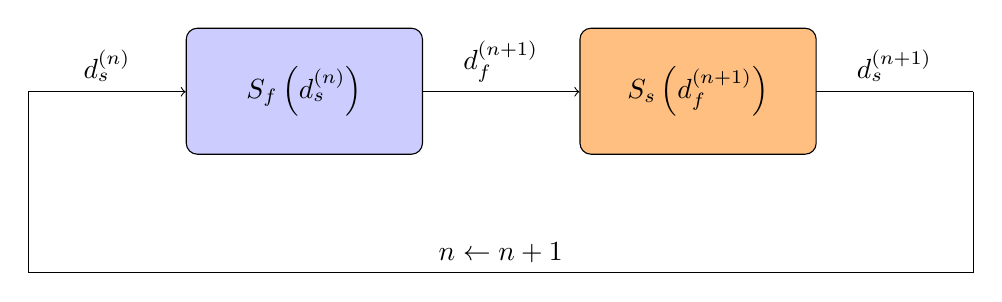
\begin{tikzpicture}[scale=1]
		\tikzstyle{solver}=[draw,rectangle,rounded corners,text centered,inner sep=10pt, anchor=south west, minimum width=3cm,minimum height=1.6cm]
		
		\node[solver,fill=blue!20] at (3,5) {$S_f\left( d_s^{(n)} \right)$};
		\node[solver,fill=orange!50] at (8,5) {$S_s\left(d_f^{(n+1)}\right)$};
		
		\draw[->] (1,5.8)-- (3,5.8) node[midway,above] {$d_s^{(n)}$};
		\draw[->] (6,5.8)-- (8,5.8) node[midway,above] {$d_f^{(n+1)}$};
		\draw[-] (11,5.8)-- (13,5.8) node[midway,above] {$d_s^{(n+1)}$};
		
		\draw[-] (13,5.8)-- (13,3.5);
		\draw[-] (1,5.8)-- (1,3.5);
		
		\draw[-] (1,3.5)-- (13,3.5) node[midway,above] {$n \leftarrow n+1$};
		
		\end{tikzpicture}
		\caption{serial explicit coupling}
		\label{fig:serial-explicit}
	\end{subfigure}
	\newline
	\centering
	\begin{subfigure}{.8\textwidth}
	\centering
	% include second image
		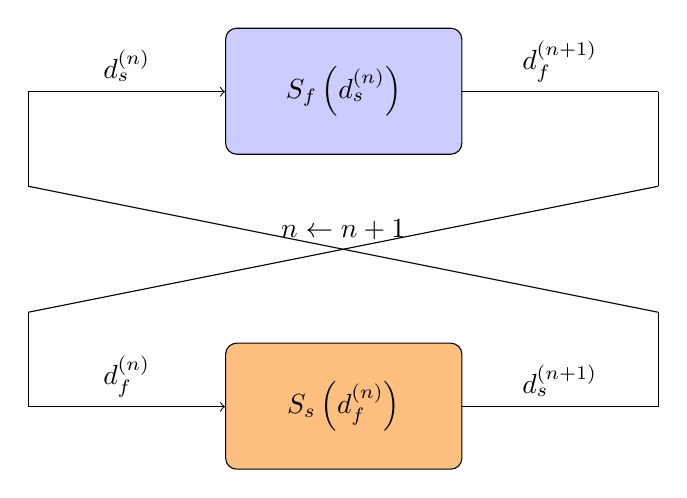
\begin{tikzpicture}[scale=1]
		\tikzstyle{solver}=[draw,rectangle,rounded corners,text centered,inner sep=10pt, anchor=south west, minimum width=3cm,minimum height=1.6cm]

		\node[solver,fill=blue!20] at (2.5,4) {$S_f\left( d_s^{(n)} \right)$};
		\node[solver,fill=orange!50] at (2.5,0) {$S_s\left(d_f^{(n)}\right)$};
		
		\draw[->] (0,4.8)-- (2.5,4.8) node[midway,above] {$d_s^{(n)}$};
		\draw[->] (0,0.8)-- (2.5,0.8) node[midway,above] {$d_f^{(n)}$};

		\draw[-] (5.5,4.8)-- (8,4.8) node[midway,above] {$d_f^{(n+1)}$};
		\draw[-] (5.5,0.8)-- (8,0.8) node[midway,above] {$d_s^{(n+1)}$};
		
		\draw[-] (0,0.8)-- (0,2);
		\draw[-] (8,0.8)-- (8,2);
		
		\draw[-] (0,3.6)-- (0,4.8);
		\draw[-] (8,3.6)-- (8,4.8);
		
		\draw[-] (8,3.6)-- (0,2) node[midway,above] {$n \leftarrow n+1$};
		\draw[-] (0,3.6)-- (8,2);

	
		\end{tikzpicture}
		\caption{parallel explicit coupling}
		\label{fig:parallel-explicit}
	\end{subfigure}
	\caption{Explicit coupling schemes}
\end{figure}

In general, an explicit coupling is not enough to regain the exact (as in the monolithic approach) solution of the problem as the matching coupling conditions between the solvers is not enforced within each time step: no balance between fluid and structural domain with respect to forces and displacements at the interface can be guaranteed (\cite{hou2012numerical}, \cite{degroote2009performance}). Nevertheless, explicit coupling yields good results if the interaction between fluid and solid is weak as in aeroelastic simulations, where in general the simulations show small displacements of the structure within a single time step and the flow field isn't much influenced by the structural displacements (\cite{farhat2006provably}).

\subsection{Implicit coupling schemes}


On the other hand, strongly (implicit) coupling techniques require an iterative method to solve the fixed-point equation that derives from enforcing the agreement of the interface variables.
The coupling conditions at the wet surface are enforced in each time step up to a convergence criterion. If the criterion is not met, another subiteration within the same time instance is computed. Therefore, the solution can approximate the monolithic solution to an arbitrary accuracy.

As in the explicit case, solvers may run in a sequential mode: the coupling is then named \textit{serial} (or staggered) and the solvers wait for each other. 

\begin{subequations}
	\begin{eqnarray}
		d_f^{(n+1),i+1} &=& S_f\left(d_s^{(n+1),i}\right) \\
		d_s^{(n+1),i+1} &=& S_s\left( d_f^{(n+1),i+1} \right)
	\end{eqnarray} 
	\label{eq:ser-imp}
\end{subequations}

Equations \ref{eq:ser-imp} show that, in contrast with explicit coupling, both solvers use interface values at time step $n+1$, but one of them uses data from previous iteration.
If run in parallel mode \cite{mehl2016parallel}, the system becomes:

\begin{subequations}
	\begin{eqnarray}
		d_f^{(n+1),i+1} &=& S_f\left(d_s^{(n+1),i}\right) \\
		d_s^{(n+1),i+1} &=& S_s\left( d_f^{(n+1),i} \right)
	\end{eqnarray} 
	\label{eq:par-imp}
\end{subequations}

At convergence, the following relation holds of serial (or \textit{Gauss-Seidel}) coupling:


\begin{subequations}
	\begin{eqnarray}
		d_s^{(n+1)} &=&  S_s\left(S_f\left(d_s^{(n+1)}\right) \right) \\
		\label{eq:ser-fp-comp}
		d_s^{(n+1)} &=& S_s  \circ S_f \left( d_s^{(n+1)} \right)
	\end{eqnarray} 
	\label{eq:ser-fp}
\end{subequations}


and the following relation holds for parallel (or \textit{Jacobi}) coupling:

\begin{equation}
	\begin{pmatrix}
		d_s^{(n+1)} \\
		d_f^{(n+1)}
	\end{pmatrix} = 
	\begin{pmatrix}
		0 & S_f \\
		S_s & 0
	\end{pmatrix} 
	\begin{pmatrix}
		d_s^{(n+1)} \\
		d_f^{(n+1)}
	\end{pmatrix}
	\label{eq:par-fp}
\end{equation}


Acceleration techniques are necessary to bring fixed point equation \ref{eq:ser-fp-comp} or \ref{eq:par-fp} to convergence. Those techniques are described in Section \ref{sec:strong-coupling}.

The two implicit schemes are shown schematically in Figures \ref{fig:serial-implicit} and \ref{fig:parallel-implicit}: \textit{accel} refers to the post-processing step implemented to speedup convergence. After every non-converged iteration, the latest stored state of the solver (\textit{checkpoint}) is reloaded and coupling iteration \textit{i} for the current time step is incremented. When the solution converges, the time step \textit{n} is incremented.


\begin{figure}[htbp!]
	\centering
	\begin{subfigure}{.8\textwidth}
		\centering
		% include first image
		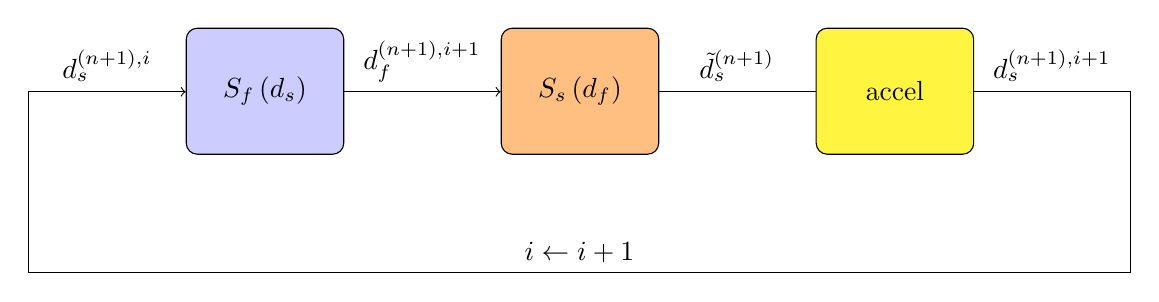
\begin{tikzpicture}[scale=1]
			\tikzstyle{solver}=[draw,rectangle,rounded corners,text centered,inner sep=10pt, anchor=south west, minimum width=2cm,minimum height=1.6cm]
			
			\node[solver,fill=blue!20] at (2,5) {$S_f\left( d_s\right)$};
			\node[solver,fill=orange!50] at (6,5) {$S_s\left(d_f\right)$};
			\node[solver,fill=yellow!75] at (10,5) {accel};
			
			\draw[->] (0,5.8)-- (2,5.8) node[midway,above] {$d_s^{(n+1),i}$};
			\draw[->] (4,5.8)-- (6,5.8) node[midway,above] {$d_f^{(n+1),i+1}$};
			\draw[-] (8,5.8)-- (10,5.8) node[midway,above] {$\tilde{d}_s^{(n+1)}$};
			\draw[-] (12,5.8)-- (14,5.8) node[midway,above] {$d_s^{(n+1),i+1}$};
			
			\draw[-] (14,5.8)-- (14,3.5);
			\draw[-] (0,5.8)-- (0,3.5);
			
			\draw[-] (0,3.5)-- (14,3.5) node[midway,above] {$i \leftarrow i+1$};
			
		\end{tikzpicture}
		\caption{serial implicit coupling}
		\label{fig:serial-implicit}
	\end{subfigure}
	\newline
	\centering
	\begin{subfigure}{.8\textwidth}
		\centering
		% include second image
		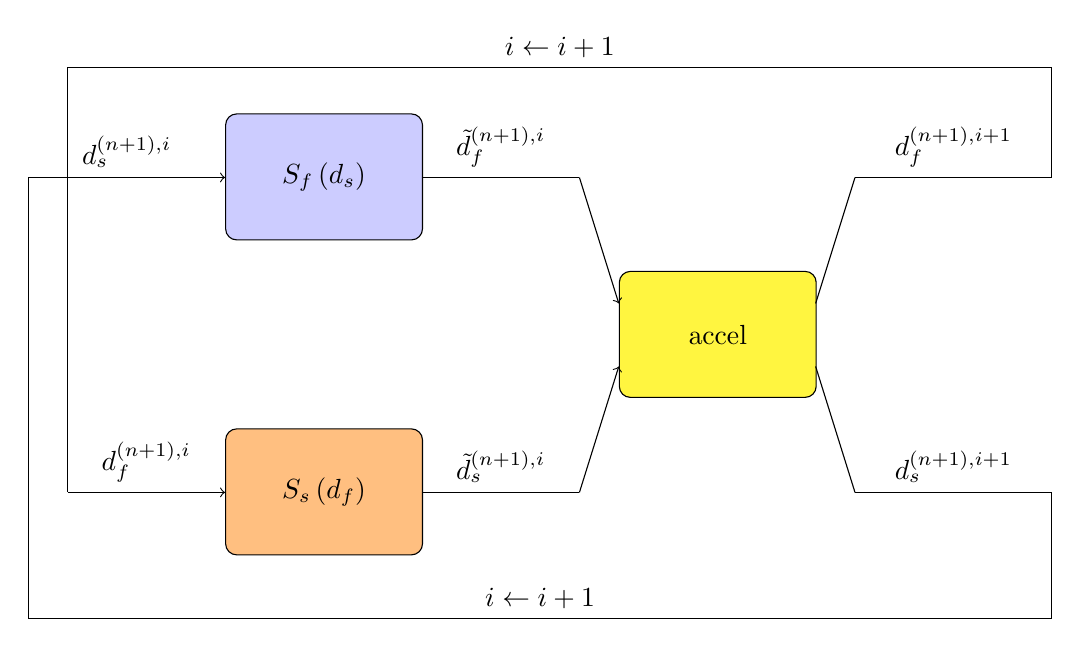
\begin{tikzpicture}[scale=1]
			\tikzstyle{solver}=[draw,rectangle,rounded corners,text centered,inner sep=10pt, anchor=south west, minimum width=2.5cm,minimum height=1.6cm]
			
			\node[solver,fill=blue!20] at (2.5,4) {$S_f\left( d_s \right)$};
			\node[solver,fill=orange!50] at (2.5,0) {$S_s\left(d_f\right)$};
			
			\node[solver,fill=yellow!75] at (7.5,2) {accel};
			
			\draw[->] (0,4.8)-- (2.5,4.8) node[midway,above] {$d_s^{(n+1),i}$};
			\draw[->] (0.5,0.8)-- (2.5,0.8) node[midway,above] {$d_f^{(n+1),i}$};
			
			\draw[-] (5,4.8)-- (7,4.8) node[midway,above] {$\tilde{d}_f^{(n+1),i}$};
			\draw[-] (5,0.8)-- (7,0.8) node[midway,above] {$\tilde{d}_s^{(n+1),i}$};
			
			\draw[->] (7,4.8)-- (7.5,3.2);
			\draw[->] (7,0.8)-- (7.5,2.4);
			
			\draw[-] (10,3.2)-- (10.5,4.8);
			\draw[-] (10,2.4)-- (10.5,0.8);

			\draw[-] (10.5,4.8)-- (13,4.8) node[midway,above] {$d_f^{(n+1),i+1}$};
			\draw[-] (10.5,0.8)-- (13,0.8) node[midway,above] {$d_s^{(n+1),i+1}$};

			\draw[-] (13,4.8)-- (13,6.2);
			\draw[-] (13,0.8)-- (13,-0.8);

			\draw[-] (13,6.2)-- (0.5,6.2) node[midway,above] {$i \leftarrow i+1$};
			\draw[-] (13,-0.8)-- (0,-0.8) node[midway,above] {$i \leftarrow i+1$};
			
			\draw[-] (0,-0.8)-- (0,4.8);
			\draw[-] (0.5,6.2)-- (0.5,0.8);

			%\draw[-] (0,0.8)-- (0,2);
			%\draw[-] (8,0.8)-- (8,2);
			
			%\draw[-] (0,3.6)-- (0,4.8);
			%\draw[-] (8,3.6)-- (8,4.8);
			
			%\draw[-] (8,3.6)-- (0,2) node[midway,above] {$n \rightarrow n+1$};
			%\draw[-] (0,3.6)-- (8,2);
			
			
		\end{tikzpicture}
		\caption{parallel implicit coupling}
		\label{fig:parallel-implicit}
	\end{subfigure}
	\caption{Implicit coupling schemes}
\end{figure}

Implicit methods are generally applicable to any kind of FSI problems, in contrast with explicit methods. When fluid and structure are strongly coupled, explicit coupling can be subject to numerical instabilities, a problem that cannot always be solved by reducing the coupling time step size \cite{van2009added}. These instabilities can be overcome by implicit methods, even if several coupling iterations may be executed every time step, until the values on both sides of the interface converge.


\section{Strong coupling algorithms}
\label{sec:strong-coupling}

As mentioned in the previous section, implicit methods require some post-processing (generally called \textit{acceleration}) techniques to to make the solution of the single time step of the coupled partitioned FSI problem converge. This requires to solve a a \textit{fixed-point equation}, in fact:

\begin{subequations}
	\begin{eqnarray}
		\label{eq:fp-def}
		H(d_s) &\coloneqq&  S_s  \circ S_f(d_s)  \\
		\label{eq:fp-2}
		d_s &=& H(d_s)  \\
		\label{eq:fp3}
		R(d) &\coloneqq& H(d) - d
	\end{eqnarray} 
	\label{eq:fp-equations}
\end{subequations}

Equation \ref{eq:fp-def} represents the composition of the solid and the fluid solution, while Equation \ref{eq:fp-2} represents the resulting fixed point equation. As the order of execution can be switched, in Equation \ref{eq:fp3}, where the \textit{residual} is defined, the input data $d_s$ is generically substituted with $d$.

The basic approach to solve the fixed point equation is to perform the corresponding ~\ac{FPI}:

\begin{equation}
	x_{i+1} = H(x_i) \quad i=1,2,\ldots
\end{equation} 

which is known to converge if the mapping \textit{H} is a contraction, but this is not the general case in FSI computations \cite{mehl2016parallel}. The way to stabilize the iterations is to perform a FPI with \textit{under-relaxation} as illustrated in the following algorithm:

\begin{algorithm}[H]
	\SetAlgoLined
	\KwResult{$d_k$}
	initialization of $d_0$\;
	k = 0\;
	$\tilde{d}_1 = S_s \circ S_f(d_0)$\;
	$r_0$ = $\tilde{d}_1 - d_0$\;
	\While{$\lVert r_k \rVert > \varepsilon$}{
		compute $d_k$ by relaxation\;
		k = k +1\;
	}
	\caption{FPI with relaxation}
\end{algorithm}

The under-relaxation is defined by:

\begin{equation}
	d_{k+1} = d_{k} + \omega \left( H(d_k)  - d_k  \right)
	\label{eq:ur}
\end{equation} 

Where $\omega$ in Equation \ref{eq:ur} is the \textit{relaxation factor}. Constant under-relaxation often leads to divergence or very slow convergence, some adaptive factor is needed, like the \textit{Aitken under-relaxation} \cite{irons1969version} which adapts the factor at each iteration:

\begin{equation}
	\omega_i = -\omega_{i-1} \frac{r_{i-1}^T \left(r_i - r_{i-1}\right)}{ \lVert r_i - r_{i-1} \rVert ^2}
\end{equation}




























\section{Interface Mesh}
\label{sec:interface-mesh}

In this section, FSI methods are classified by means of two different mesh treatment procedures: conforming
or non-conforming techniques. The basic question is, whether fluid and solid mesh need to align
with each other at the FSI interface or not. Unless stated otherwise, the explanations of this section are
taken from [20]. Note that some aspects of conforming mesh methods are already included in the previous
sections without explicitly mentioning so, in order to develop a better understanding of partitioned FSI
simulations.
Conforming mesh methods usually consist of three major subtasks, namely computation in the fluid and
solid domain, as well as interface and mesh movement. They require both fluid and structural meshes
to conform to the wet surface, because the coupling conditions are applied via the interface as physical
boundary conditions for the respective domains. This does not necessarily imply node-to-node matching
of fluid and structure meshes at the interface. This must hold for all time instances, which means that
both fluid and structural grids need to be moved in case deformations of the solid appear. This is a
simple task for the solid mesh, since it is usually expressed in a Lagrangian fashion anyway. However, as
a typical Eulerian fluid mesh would not follow the interface motion, the necessity of the ALE method as
discussed in Section 2.2.3 becomes apparent. Also, mesh smoothing techniques need to be introduced in order to prevent quality losses of the fluid mesh in terms of distorted elements. These irregularities lead
to accuracy loss in simulations. In Figure 3.5, a conforming mesh is shown at two different points in time.
At the first instance (Figure 3.5a) the solid is undeformed and therefore, also the fluid mesh remains in
its initial configuration. In contrast, at the second point in time (Figure 3.5b) the solid is deformed and
the fluid mesh conforms to the displaced wet surface. Consequently, also mesh smoothing is applied.
There is a wide variety of such mesh updating procedures. Some common techniques compute the mesh
movement by considering mesh edges as springs ((torsional) spring analogy), solving the Laplace equation
or solving a pseudo-structural system of equations (see e.g. [18], [43], [20] and their respective references
for further explanations of these techniques). Conforming mesh strategies are widely, but not exclusively
used in partitioned FSI approaches. Furthermore, they typically also utilize the ALE method ([20]).
In contrast, in non-conforming mesh strategies all interface conditions are directly imposed as constraints
on the flow and structural governing equations. Therefore, it is possible to use non-conforming meshes
for fluid and solid domains as they remain geometrically independent from each other. Thus, also mesh
smoothing techniques are obsolete [43]. Figure 3.6 depicts such a situation. By analogy with Figure 3.5,
again the initial configuration (Figure 3.6a) and an instance when the solid is deformed (Figure 3.6b) are
shown. It is clearly visible that the fluid mesh does not conform to the wet surface as all nodes stay at
the same position regardless of the solid deformation.
This approach is mostly used in immersed methods. The considerations in this section are limited to them,
as they are also very common for FSI simulations. Coupling is imposed via additional force-equivalent
terms appearing in the model equations of the fluid, enforcing the kinematic and dynamic conditions.
These FSI forces are computed from the structural model, which is dealt with separately together with
tracking the position of the interface. The forces represent the effects of a boundary or body being
immersed in the fluid domain (leading to immersed boundary and immersed domain methods). A purely
Eulerian mesh can be applied to the whole computational domain for solving the fluid equations, since
the force-equivalent terms are dynamically added in a spatially specific manner to those locations, which
are currently occupied by the structure. After solving the fluid equations, forces exerted on the solid at
the wet surface are computed and used as input for the structural solver, which still employs a Lagrangian
mesh. Subsequently, the deformation of the solid material is calculated and the displacement of the FSI
interface is fed back to the fluid model in form of updated force-equivalent terms ([31], [20], [43]).

\section{Stability: Added Mass Effect}
\label{sec:addedd-mass}

To conclude this chapter about computational aspects of FSI simulations, the AME is briefly described.
Explanations of this effect can be found in a great variety throughout FSI literature, typically explicated
for specific solver strategies or flow regimes (see e.g. [5], [42], [15], [2]). Therefore, in the scope of
this thesis only a short phenomenological introduction to the concept of added mass and numerical
problems arising from it is given. However, this suffices to focus on both weakly and strongly coupled partitioned approaches, which are practically relevant in this thesis. The AME is inherent to partitioned
FSI approaches as the single-physics fields are not continuously coupled but interaction only occurs at a
finite number of discrete time instances, when coupling quantities are exchanged.
As already mentioned in Section 2.3.3, there can be no gaps between structure and fluid. Also their
respective particles cannot occupy the same spatial locations simultaneously. Thus, if the solid is moved,
also fluid particles move. Changing the state of motion of the structural component consequently requires
taking into account inertial effects not only of the solid itself, but also of the surrounding fluid, which
artificially rests for the span of a single structure solver time step. In more descriptive words: Moving the
solid also implies moving fluid particles close to the solid. Therefore, the structure behaves more inert
due to artificially added mass ([42], [2]). Since inertia is dependent on mass and therefore density, the
% AME is also. More precisely, it is dependent on the ratio (MA) of structural (S) und fluid density (F )
([42], [5]):
%MA = S F : (3.1)
This ratio is often used to describe how strong the interaction between solid and fluid is. For cases, in
%which the solid density is much higher than the fluid density (MA  1), this effect does not dominantly
influence the FSI problem (weak interaction). But as fluid and structure densities approach each other
%(MA  1) or the fluid becomes even denser than the solid (MA < 1), its consideration is crucial (strong
interaction) and imposes stability limits on partitioned solution techniques ([5], [42], [2]). Note that the
AME is not only governed by the density ratio of Equation 3.1 but also by geometric properties of the
problem, the stiffness of the solid ([5]) and the speed of sound in the flow domain ([42]). Nonetheless,
for the sake of simplicity and intuitiveness, explanations in this thesis are mostly limited to the density
ratio.
In general, the AME is of bigger concern for incompressible flows than for compressible regimes. From
a physical point of view, deformations of the structural domain can be interpreted as perturbations for
the flow field. In compressible flows the speed of sound (speed at which perturbations propagate through
the flow) is finitely large. Thus, the influence of a geometrical change of the fluid domain caused by
deformations of the solid is locally limited during a certain period of time. In contrast, in incompressible
flows the speed of sound is infinitely large, hence all perturbations propagate through the flow without
time delay. Therefore, regardless of how much time has passed since a perturbation, the whole flow field
is directly affected ([42], [5]).
In the following it is assumed that a weakly coupled algorithm allows computation of the fluid and solid
solution only once per time step. In addition, coupling data is also exchanged once per time instance. In
contrast, a strongly coupled solver does the same at least twice per time increment (for a reminder see
Section 3.2 and compare Figure 3.4). As can be shown, in the compressible case a more dominant AME
can be compensated for by reducing the time step size of strongly coupled, partitioned solution algorithms.
This however, does not hold for the incompressible regime, where even in the limit of vanishing time step
size strongly coupled, partitioned algorithms might fail ([42]). These observations are consistent with the
above mentioned physical explanation.
First of all, considering compressible flows, indeed, the lack of repeated subiterations in weakly coupled
partitioned techniques leads to a strict limit for the density ratio (of Equation 3.1) due to the fact that
the interface conditions are not enforced and energy balance at the wet surface is generally not given.
If that limit is exceeded the algorithm fails due to instability ([2]). Likewise, in such a case a strongly
coupled partitioned algorithm converges slowly, resulting in possibly many necessary subiterations, which
is computationally costly. Yet it does not become unstable, given that the time step size is chosen sufficiently
small. Reducing the time step size to an arbitrarily small extent cannot stabilize a weakly coupled
approach if the stability criterion on the density ratio is not met ([15]). Conversely, the convergence
rate of strongly coupled algorithms increases by the same factor, by which the time step size decreases,
meaning that in the limit of vanishing time step size the monolithic solution is obtained ([5], [42]).
In the incompressible case however, a strict stability limit exists for both weakly and strongly coupled
algorithms. It is independent of the size of time increments1. Furthermore, in order for an implicit
method to achieve the monolithic solution (assuming its convergence is given, i.e. the before mentioned
stability limit is not exceeded) the number of subiterations must be increased as time step size decreases
([15], [42]).